\subsection{Ohrenzerlegung}

Es sei nur dann ein Graph \textit{G(V,E)} mit $|E|>=2$, der 2-Vertex-verbunden ist, gegeben, wenn es eine offene Ohrenzerlegung gibt. Jede Ohrenzerlegeung definiere eine Kreisbasis.

\begin{itemize}
	\item \textbf{\textit{Kreisbasis:}} \newline Ein Ohr Sei ein maximaler Pfad P, $|P| >= 1$, so dass P nur an Endpunkten Kanten aus $E\notin P$ berührt. Die Knoten in P, die keine Endknoten sind haben immer Grad $deg = 2$.
	\item \textbf{\textit{offene Ohrenzerlegung}}\newline Eine Folge von Ohren $P_1, P_2, ..., P_k$ist eine offene Ohrenzerlegung, wenn $P_1$ ein Kreis, $P_k$ und alle anderen $P_i$ Ohren in $G_i = G_{i+1} \setminus P_{i+1}$ 
\end{itemize}
\subsubsection{Algorithmus der Ohrenzerlegung}
\begin{itemize}
	\item[1] Finde Spannbaum T für G und wähle eine Wurzel
	\item[2] Für jede Kante (u,v), die nicht Teil des Spannbaums ist, finde den \textit{common lowest ancestor} der Knoten u und v.
	\item[3] Fuer jede Kante (u,v) soll die Hauptkante (w,x) gefunden werden, wobei (u,v) und (w,x) Teil eines Kreises sind und (w,x) einen \textit{lowest common ancestor} so nah wie moeglich an der Wurzel haben und (w,x) $\notin$ von T ist.
	\item[4] Für alle (w,x) die nicht aus dem Spannbaum sind, trenne alle Kanten mit gleichem Wert ab. Diese Kanten bilden ein Ohr.
	\item[5] Ordne die Ohren nach ihrem Gewicht. 
\end{itemize}
\subsection{Unabhaengigkeitssysteme und Matroide}

Viele \textit{Greedy Probleme} lassen sich mittels Matroiden beschreiben (insbesondere Graphenprobleme).\newline

\begin{itemize}
	\item \textbf{\textit{Unabhaengigkeitssystem}} \newline Ein Unabhaengigkeitssystem ist ein Paar $M = (S,l)$ mit endlicher Menge $S$ und $l <= P_S(S)$ (Powerset von S). Es besitzt folgende Eigenschaften:
	\begin{itemize}
		\item[1] $\emptyset = {} \in l$ $\rightarrow$ Die leere Menge ist unabhängig
		\item[2] $x \subseteq Y \in l$ $\rightarrow$ Erblichkeitseigenschaft
	\end{itemize}
	Die Elemente $x \in l$ und $y \in P_S(S) \setminus l$ sind unabhängig. \newline
	$\rightarrow$ Kostenfunktion C: S $\rightarrow \mathbb{R}$ 
\end{itemize}
\textit{Austauscheigenschaft:} \newline Falls $A \in l, B \in l, |A| < |B|$, dann $\exists x, x \in B \setminus A: A \cup \{x\} \in l$
\begin{itemize}
	\item[] \textit{Matroid}\newline Ein Unabhängigkeitssystem sei ein Matroidfalls die Eigenschaften eines Unabhängigkeitssystems und die Austauscheigenschaft erfüllt sind.
	\item[] \textit{grafischer Matroid}\newline Ein graphischer Matroid $M_G = (S_G,l_G) mit S_G = E(G)$
	\begin{itemize}
		\item[$\rightarrow$] für $A \subseteq S_G: \in l_G \leftrightarrow$ A ist kein Kreis
		\item[$\rightarrow$] Menge an Kanten ist nur dann unabhängig, wenn G' = (V(G),A) einen Wald bilden $\rightarrow$ G' bildet keinen Kreis
	\end{itemize}
\end{itemize}

\textit{Extension:} \newline Sei M = (S,l) und x $\notin$ A gegeben, so sei l eine Erweiterung von A, falls $A \cup \{x\}$ unabhängig ist. ($A \cup \{x\}\in l$) \newline  $\rightarrow$ Kante l ist eine Erweiterung, falls $A \cup \{x\}$ keinen Kreis bilden. \newline 

\textit{Maximalität:} \newline $A \in l$ ist maximal, falls es keine Erweiterung für A gibt. \newline

\textbf{Theorem} \newline Alle maximal unabhängigen Teilmengen in einem Matroid haben die selbe Größe.

\textbf{Beweis} \newline Wenn das Theorem nicht gilt, so wären die maximal unabhängigen Elemente A und B mit $|A| < |B|$. Damit würde die Austauscheignschaft zeigen, dass x abhängig von A ist: $\exists x: B\setminus A: A \cup \{x\}$. $\rightarrow$ Beweis durch Widerspruch\newline

\textbf{Beispiel}\newline Gegeben Graph G gilt, dass alle Spannbäume, die gleiche Anzahl an Kanten haben: $|E| = |V| - 1$. \newline
\begin{itemize}
	\item \textbf{\textit{gewichtetes Matroid}} \newline Ein Matroid M=(S,l) ist gewichtet, falls es eine Gewichtsfunktion $w(x) > 0 \forall x \in S$ gibt. $\rightarrow$ w(A), $A \subseteq S mit w(A) = \sum_{x \in A} w(x)$.
\end{itemize}

\subsubsection{Greedy Algorithmen auf Matroiden}

Gegeben sei M(S,l). Finde $A \in l$, sodass w(A) maximal ist.\newline

\textbf{Beispiel:} Minimallänge Spannbäume mit \newline $w'(x) 0 w_0 - w(x)$ mit $w_0 = max_{x}(w(x)) + \epsilon$ \newline

\textbf{\textit{Greedy-Algorithmus}}
\begin{itemize}
	\item[1] $A \leftarrow \{ \}$
	\item[2] sortiere S[M] nach absteigendem Gewicht
	\item[3] $\forall x \in S[M] \{$ if $A\cup \{x\} \in l$: then A $\leftarrow A \cup \{x\}\}$
	\item[4] return A
\end{itemize}

\textbf{Theorem} \newline A ist die optimale Lösung des Greedy-Algorithmus \newline

\textbf{Beispiel} \newline Betrachte und bilde Kreisbasen L1 oder L2. L1 hat insgesamt weniger Knoten als L2 und ist somit eine bessere Lösung. C(G) ist ein Matroid mit den Elementgewichten $|C| \rightarrow$ diese definieren S $\rightarrow$ die minimalen Kreisbasen werden in polynomieller Zeit in $|C|$ berechnet.
\subsubsection{Horton-Algorithmus (1972)}
\begin{itemize}
	\item[1]Konstruiere die kürzesten Pfadbäume mittels Matroide. 
	\item[2]Extrahiere die fundamentalen/minimalen Kreise der Pfadbäume.
\end{itemize}
$\rightarrow$ Berechnung ist polynomiell abhängig von $|V|$
\begin{itemize}
	\item essentielle Kreise sind Kreise, die in allen minimalen Kreisbasen vorkommen. 
	\item relevante Kreise sind Kreise, die in mindestens einer minimalen Kreisbasenlösung vorkommen.
	\item Falls C nicht in ein einfacher Kreis ist, dann ist C keine minimale Kreisbase.
\end{itemize}

\subsection{Graphen in der Ebene und planare Graphen}
\textbf{Topologie}
\begin{itemize}
	\item euklidische Ebene: $\mathbb{R}^2$ 
	\item Liniensegmente \{ p+x(q-p)\} mit p,q $\in \mathbb{R}^2$ und $p \neq q$
	\item homöomorphisch (bijektive stetige Abbildung) zum Einheitskreis
	\item Polygonzug (zusammenhängende Folge von Kanten)
\end{itemize}
\textbf{\textit{Theorem}: Jordan'scher Kurvensatz}\newline
Für jedes Polygon $P \subseteq \mathbb{R}^2$ hat $\mathbb{R}^2\notin P$ zwei Regionen, wobei P die Grenze bildet\newline $\rightarrow$ definiertes außen und innen \newline
\textbf{Lemma}\newline
Seien $P_1, P_2, P_3$ Polygonzüge mit den Endpunkten x und y, so hat $\mathbb{R}^2 \notin \{ P_1 \cup P_2 \cup P_3\}$ drei Facetten mit den Grenzen $P_1, P_2, P_3$ (ohne die Endpunkte x und y): 
\begin{itemize}
	\item{} $b_1 := P_1 \cup P_2$
	\item{} $b_2 := P_1 \cup P_3$
	\item{} $b_3 := P_2 \cup P_3$ 
\end{itemize}
$\rightarrow$ falls $P_4$ ein Polygonzug zwischen $\dot{P_1}$ und $\dot{P_3}$ mit $\dot{P_4}, \dot{P_3} \subset \mathbb{R}^2 \notin \{ P_1 \cup P_3\}$ ist, so schneiden sich $P_4 und P_2 (\dot{P_4} \cap \dot{P_2})$ \newline

\textbf{\textit{Graph in Ebene:}} \newline
Ein Graph in der Ebene (V,E) hat folgende Eigenschaften
\begin{itemize}
	\item[1] $V \subset \mathbb{R}$
	\item[2] Jede Kante sei ein Polygonzug zwischen zwei Knoten
	\item[3] unterschiedliche Kanten haben unterschiedliche Mengen von Knoten
	\item[4] das innere einer Kante enthält keinen Knoten und keinen Punkt einer anderen Kante 
\end{itemize}
somit ist ein Graph in der Ebene \textit{kreuzungsfrei} \newline

\textbf{\textit{Facette}}\newline
Falls G ein Graph in der Ebene ist, so sind die Regionen $\mathbb{R}^2 \notin G$ die Facetten. Die äußere Facette liegt außerhalb des Graphen und die anderen Facetten liegen per Definition innerhalb. \newline

\textbf{Lemma} \newline
Sei G ein Graph in der Ebene $f \in F(G)$ eine Facette und $H \subseteq G$ ein Subgraph, so gilt:
\begin{itemize}
	\item H hat eine Facette f' mit f' $\subseteq$ f
	\item Falls der Rand von f $\subset$ H ist, dann ist f' = f
\end{itemize}
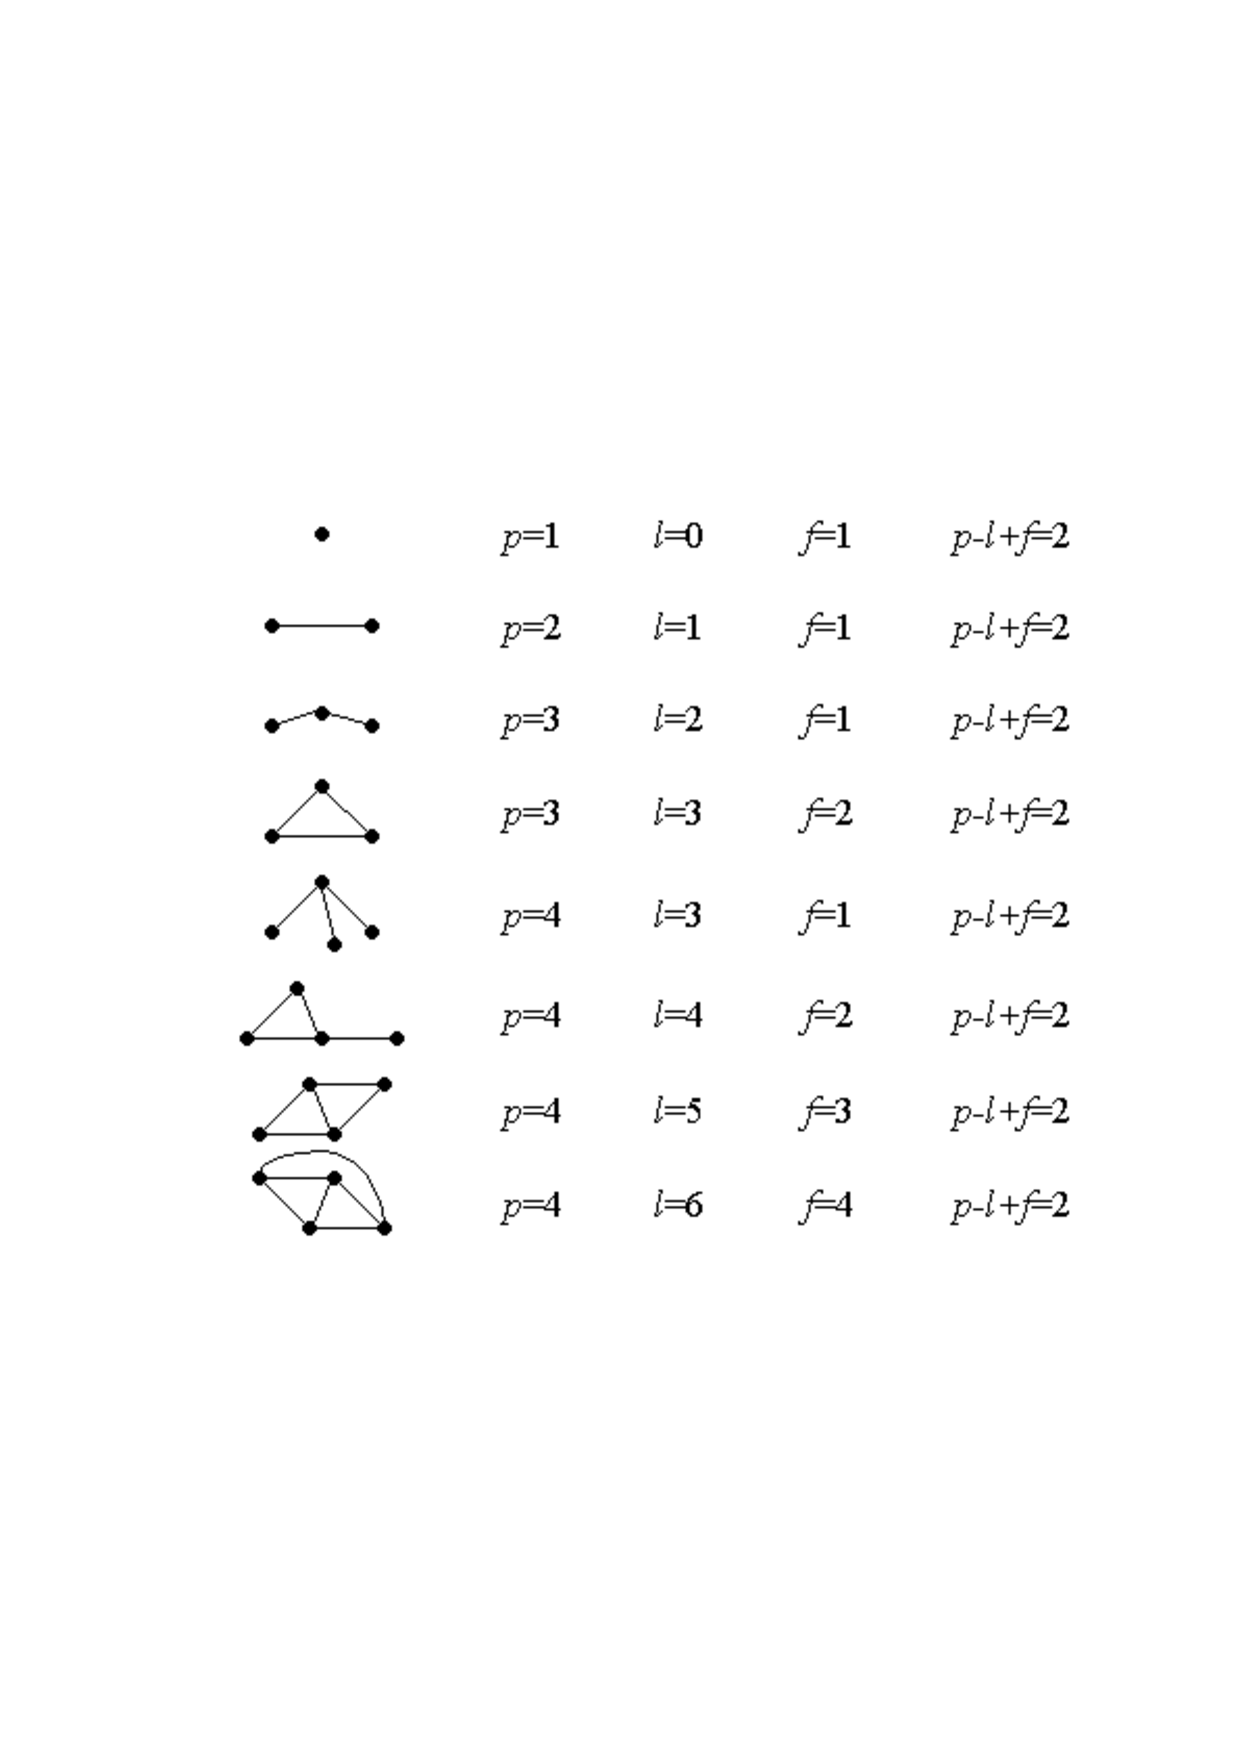
\includegraphics[scale=0.5]{planareGraphenElementar}\newline

\textbf{\textit{Theorem:} Eulersche Formel} \newline
Sei G ein verbundener Graph in der Ebene mit n Knoten, m Kanten und l Facetten, so gilt: \textbf{n - m + l = 2} \newline

\textbf{Beweis} \newline
Sei n fixiert $rightarrow$ induziere über m.
\begin{itemize}
	\item[$if m < n -1:$] Graph ist nicht verbunden
	\item[$if m = n -1:$] Graph ist ein Baum
	\item[$if m \ge n:$] Sei $e \in E(G)$ Kante auf einem Kreis, dann ist G' = G-e $\rightarrow$ e liegt auf der Grenze zweier Facetten $f_1 und f_2$ von G und es gibt eine Facette $f_e$ von G', die $\dot{e}$ enthält. 
\end{itemize}
Zeige, dass $F(G) \notin \{f_1, f_2\} = F(G') \notin \{f_e\}$, womit G' eine Facette und eine Kante weniger hat als G. \newline
$\rightarrow$ Das entfernen einer Kante kombiniert 2 Facetten \newline
$\rightarrow$ Fügt man eine Kante hinzu so wird auch eine Kante hinzugefügt \newline
$\rightarrow$ $|V'|=|V|+1$ und $|E'|=|E|+1$ $\rightarrow$ q.w.e.d. \newline
  
\textbf{Korollar 1}
\begin{itemize}
	\item[1)] Ein Graph in der Ebene mit $n \ge 3$ Knoten hat maximal 3n - 6 Kanten
	\item[2)] Jede Triangulation mit n Knoten hat genau 3n - 6 Kanten 
\end{itemize}
\textbf{Korollar 2(nach Kuratowski)} \newline
Ein Graph in der Ebene hat weder $K_5$ noch $K_{3.3}$ als topologischen Minor ($K_5$ und $K_{3.3}$ sind nicht mehr kreuzungsfrei zeichenbar).\newline
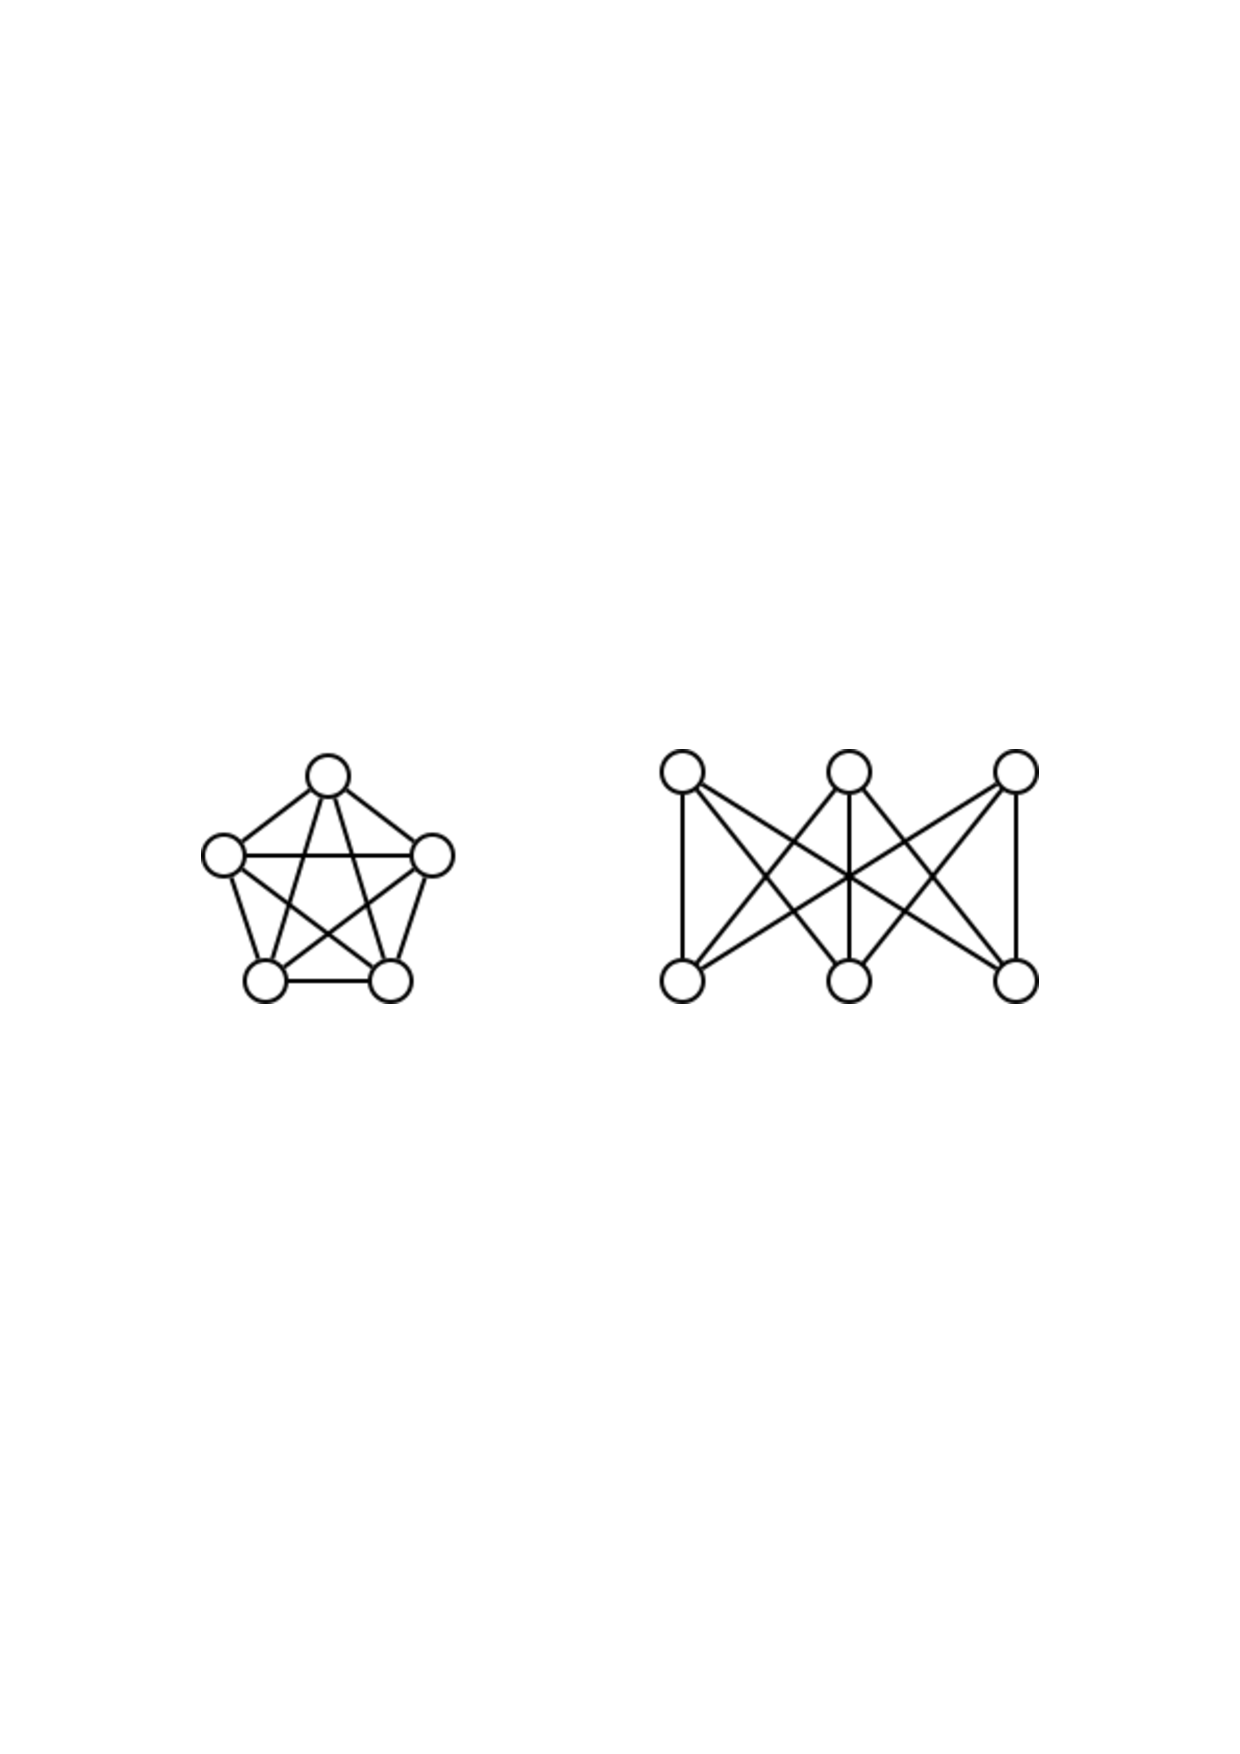
\includegraphics[scale = 0.5]{K33+K5.pdf} \newline
\textbf{\textit{Minor}}\newline
H ist ein Minor von G, falls G in H durch folgende Operationen transformiert werden kann:
\begin{itemize}
	\item G - e, e $\in$ E(G)
	\item G-v, v $\in$ V(G) (hierbei werden auch nichtverbundene Kanten gelöscht)
	\item Kontraktion von e $\in$ E(G) mit e = {u,v}, u,v $\in$ V(G), wobei u,v zu einem Knoten vereinigt werden und dieser zu allen Nachbarn inzident wird.
\end{itemize}
\textbf{\textit{planarer Graph}} \newline
Ein Graph G sei planar, wenn er folgende Eigenschaften erfüllt: 
\begin{itemize}
	\item Eine endliche Anzahl von Facetten bildet eine Kreisbasis
	\item jede Kante, die zwei Kreisen zugehörig ist, heißt innere Kante
	\item jede Kante, die einem Kreis zugehörig ist, heißt äußere Kante
\end{itemize}
\textbf{\textit{2-Basis}}\newline
Jede Kante ist genau 2 mal in den Kreisbasen vertreten.\newline
 
\textit{Konstruktion 2-Basis}
\begin{itemize}
	\item F = $\oplus_{c \in B}c$ Rand der äußeren Facette (äußerer Rand)
	\item 2-Basis = $B \cup F$ 
\end{itemize}
\textbf{\textit{Satz von Mc Lane}}\newline
G ist planar, wenn G auch eine 2-Basis hat.

\textbf{Beweis Satz von Mc Lane}\newline
\begin{itemize}
	\item[1] B sei 2-Basis von G und G sei nicht planar 
	\item[] nach Kuratowski ist Subdivision von $K_5$ oder $K_{3,3}$ $H \subset G$ möglich \newline Behauptung: $\rightarrow$ H hat ebenfalls eine 2-Basis \newline
	
	\item[2] $G \notin e, \forall e$ hat eine 2-Basis
	\item[] es ist nur in einem Kreis $C \in B$ vorhanden, womit $B \notin C$ entsteht.
	\item[] e ist in zwei Kreisen vorkommend, womit $B \notin \{C_1, C_2\} \cup \{ C_1 \oplus C_2\}$ eine 2-Basis ist \newline $\rightarrow$ somit haben alle Teilgraphen eine 2-Basis. Da die Behauptung belegt ist, wird ein Widerspruch 
\end{itemize}
\textit{zyklometrische Zahl:} Die Anzahl der Bassiselemente einer Kreisbasis nennt man zyklometrische Zahl.\newline

\textbf{\textit{Beispiel:} vollständiger Graph $K_5$} \newline
\begin{itemize}
	\item $|V| = 5 ; |E| = 10$
	\item 2-Basis mit 5 inneren und 5 äußeren Kanten
	\item $\mu(K_5)$ = -5 + 10 +1 = 7
	\item 2-Basis hat demnach (2n -6)*7 Kanten = 21 Kanten $\rightarrow$ \newline \textbf{falsche Aussage}
\end{itemize}	
\textbf{\textit{Beispiel:} bipartiter Graph $K_{3,3}$} \newline
\begin{itemize}
	\item $|V| = 6 ; |E| = 9$
	\item $\mu(K_{3,3})$ = -6 + 9 +1 = 4
	\item 2-Basis hat demnach (2n -6)*4 Kanten = 20 Kanten $\rightarrow$ \newline \textbf{falsche Aussage}
\end{itemize}
\textbf{Planaritätstest}
\begin{itemize}
	\item[1] zähle die Kanten 
	\item[2] Tiefensuche $\rightarrow$ Konstruiere einen Spannbaum
	\item[3] Teste für Kanten e $\leftarrow G \notin T$, ob $K_5$ oder $K_{3,3}$ entsteht.
\end{itemize}

\subsection{Färbung von Graphen}
\textbf{Vertexfärbung}\newline
Zwei durch eine Kante verbundene Knoten haben unterschiedliche Farben. \newline
Beispiel wäre eine Landkarte auf der mit so wenig wie möglich Farben die Länder ausgemalt werden, ohne zwei benachbarte Länder gleichfarbig zu haben. Hierbei entspricht jede Facette einen Knoten.\newline
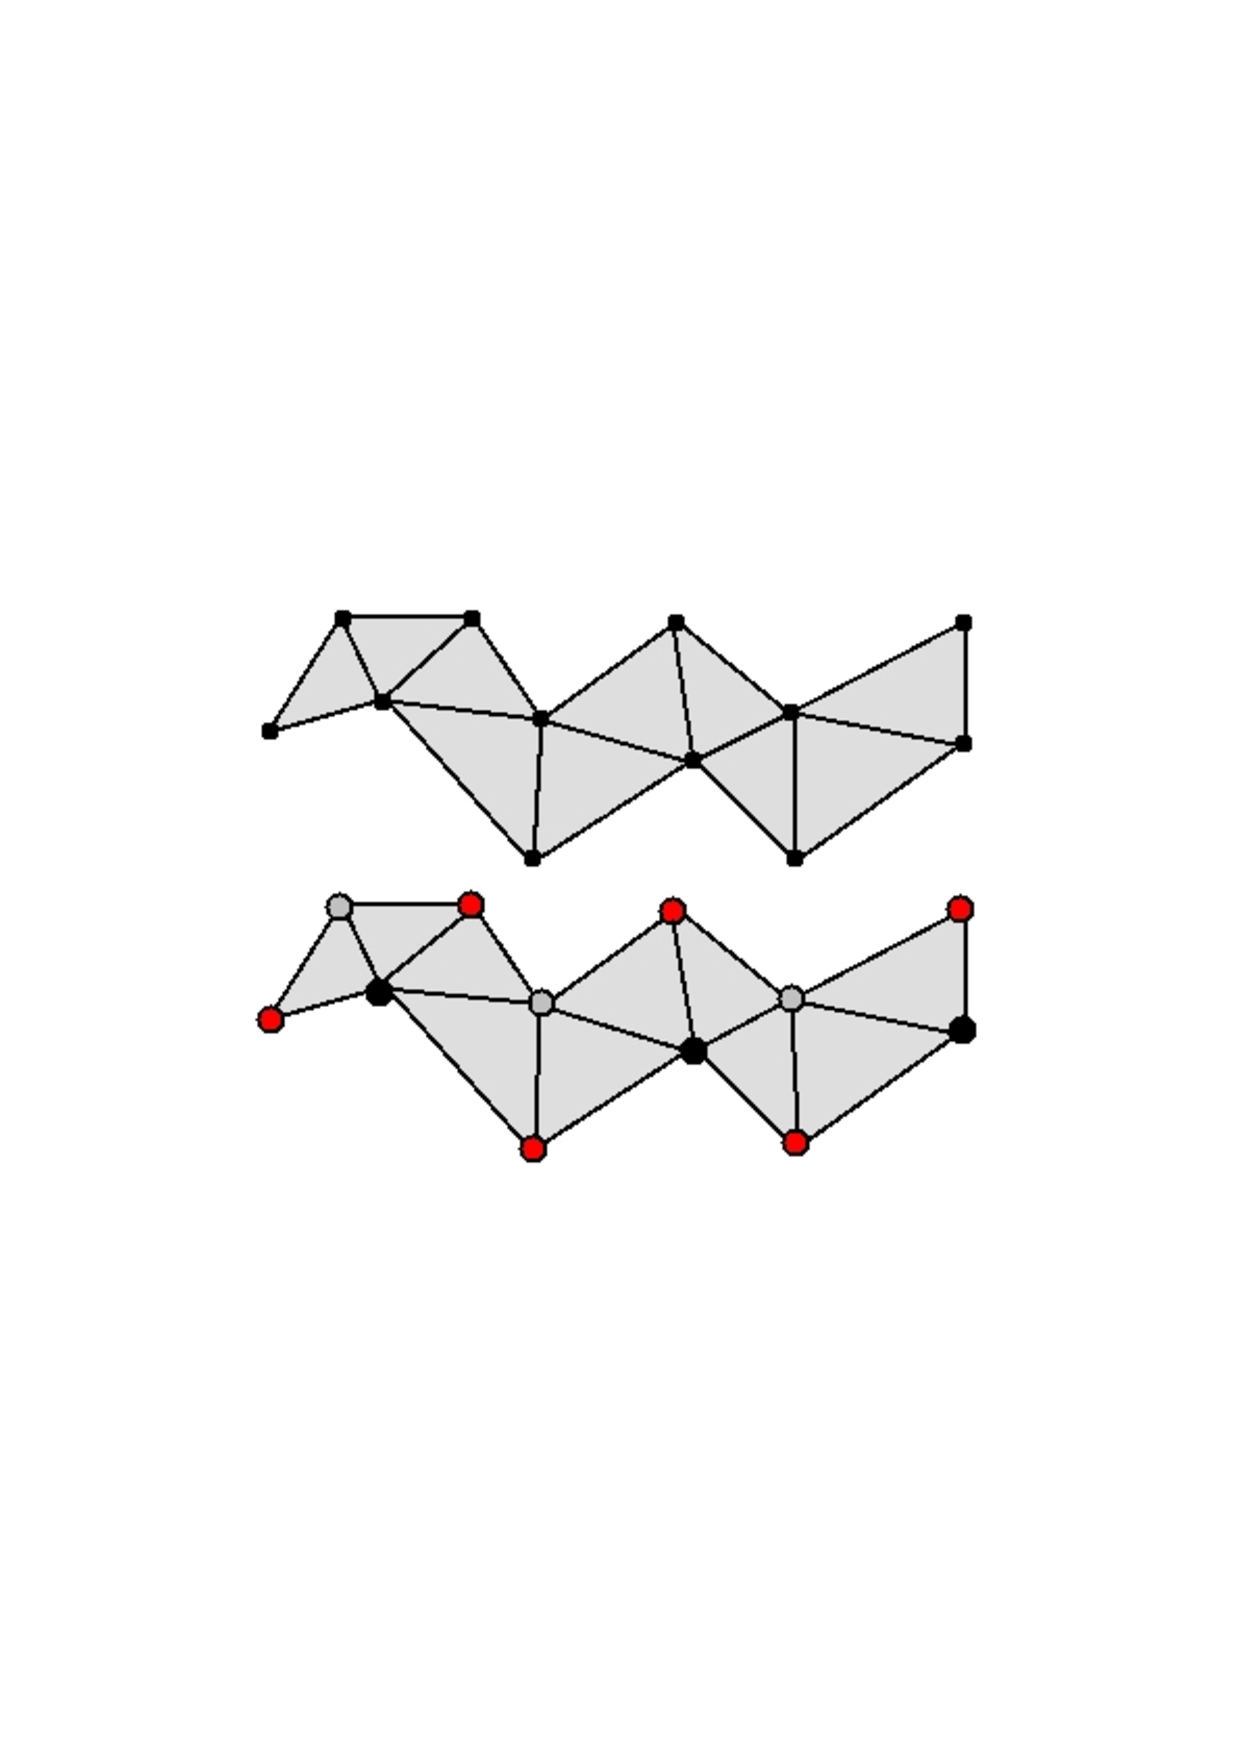
\includegraphics[width=0.4\textwidth]{Vertexfaerbung}